
%%%%%%%%%%%%%%%%%%%%%%%%%%%%%%%%%%%%%%%%%%%%%%%%%%%%%%%%%%%%%%%%%%%%%%
% Math cheat sheet
%
% Source: Felix Erlacher
%
% Date: 2014-11-10
% 
%%%%%%%%%%%%%%%%%%%%%%%%%%%%%%%%%%%%%%%%%%%%%%%%%%%%%%%%%%%%%%%%%%%%%%

\documentclass[8pt, a4paper,landscape]{article}
\usepackage{extsizes}
\usepackage{tabularray}
\usepackage{amssymb,amsmath,amsthm,amsfonts, dsfont}
\usepackage{multicol,multirow}
\usepackage{calc}
\usepackage{ifthen}
\usepackage[utf8]{inputenc}
\usepackage{graphicx}
\usepackage[landscape]{geometry}
\usepackage[colorlinks=true,citecolor=blue,linkcolor=blue]{hyperref}


\ifthenelse{\lengthtest { \paperwidth = 11in}}
    { \geometry{top=.5in,left=.5in,right=.5in,bottom=.5in} }
	{\ifthenelse{ \lengthtest{ \paperwidth = 297mm}}
		{\geometry{top=0.5cm,left=0.5cm,right=0.5cm,bottom=0.5cm} }
		{\geometry{top=0.5cm,left=0.5cm,right=0.5cm,bottom=0.5cm} }
	}
\pagestyle{empty}
\makeatletter
\renewcommand{\section}{\@startsection{section}{1}{0mm}%
                                {-1ex plus -.5ex minus -.2ex}%
                                {0.5ex plus .2ex}%x
                                {\normalfont\large\bfseries}}
\renewcommand{\subsection}{\@startsection{subsection}{2}{0mm}%
                                {-1explus -.5ex minus -.2ex}%
                                {0.5ex plus .2ex}%
                                {\normalfont\normalsize\bfseries}}
\renewcommand{\subsubsection}{\@startsection{subsubsection}{3}{0mm}%
                                {-1ex plus -.5ex minus -.2ex}%
                                {1ex plus .2ex}%
                                {\normalfont\small\bfseries}}
\makeatother
\setcounter{secnumdepth}{0}
\setlength{\parindent}{0pt}
\setlength{\parskip}{0pt plus 0.5ex}
% -----------------------------------------------------------------------

\title{Quick Guide to LaTeX}

\begin{document}

\raggedright
\footnotesize


\begin{multicols}{4}
    \setlength{\premulticols}{1pt}
    \setlength{\postmulticols}{1pt}
    \setlength{\multicolsep}{1pt}
    \setlength{\columnsep}{1pt}

    \section{Vektoren}
    \subsection{Inneres Produkt / Skalarprodukt}
    \begin{tblr}
        {
            colspec = {l Q[l]},
            rowsep  = {5pt},
            colsep  = {2pt},
        }
        \textbf{$\mathbb{R}$}         & $<\vec{a},\vec{b}> = \sum_{i = 1}^{n} = a_i b_i$                                                          \\
        \textbf{$\mathbb{C}$}         & $<\vec{a},\vec{b}> = \sum_{i = 1}^{n} = a_i b_i$                                                          \\
        \textbf{Positivität:}         & $<\vec{a},\vec{b}> \geq 0$                                                                                \\
                                      & a = 0 oder b = 0 $\rightarrow$ $<\vec{a},\vec{b}> = 0$                                                    \\
        \textbf{Symmetrie:}           & $<\vec{a},\vec{b}> = <\vec{b},\vec{a}>$ für $\mathbb{R}$                                                  \\
                                      & $<\vec{a},\vec{b}> = <\overline{\vec{b},\vec{a}}>$ für $\mathbb{C}$                                       \\
        \textbf{Linearität:}          & $<\vec{a},\textit{k}\vec{b}+\textit{h}\vec{c}> = \textit{k}<\vec{a},\vec{b}>+\textit{h}<\vec{a},\vec{c}>$ \\
        \textbf{Normalisierung:}      & $<\vec{a},\vec{a}> = ||\vec{a}||^2$                                                                       \\
                                      & 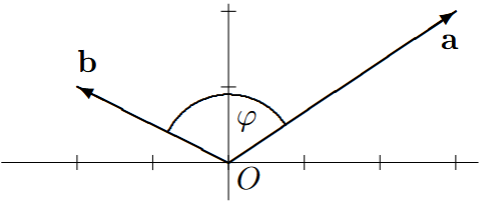
\includegraphics[width=0.1\textwidth]{figures/cosskalar.png}                                              \\
        \textbf{Matrix $\mathbb{R}$}  & $<\vec{a},\textit{A}\vec{b}> = <\textit{A}^T\vec{a},\vec{b}>$                                             \\
        \textbf{Matrix $\mathbb{C}$}  & $<\vec{a},\textit{A}\vec{b}> = <\overline{\textit{A}^T}\vec{a},\vec{b}>$                                  \\
        \textbf{Orthogonalität:}      & $<\vec{a},\vec{b}> = 0$ man schreibt $\vec{a} \perp \vec{b}$                                              \\
        \textbf{Parallelität:}        & $\vec{a} =\textit{k}\vec{b}$ oder $\vec{b} =\textit{k}\vec{a}$                                            \\
        \textbf{Winkel:}              & $<\vec{a},\vec{b}> = ||\vec{a}|| ||\vec{b}|| \cos(\alpha)$                                                \\
                                      & $\cos(\alpha) = 0$ $\alpha = 90°$ für  $\vec{a} \perp \vec{b}$                                            \\
        \textbf{Pythagoras:}          & $||\vec{a}||^2 + ||\vec{b}||^2 = ||\vec{a}+\vec{b}||^2$ für  $\vec{a} \perp \vec{b}$                      \\
        \textbf{Zerlegung}            & $\vec{a} = \vec{a}_{\perp}$ + $\vec{a}_{\parallel}$                                                       \\
                                      & 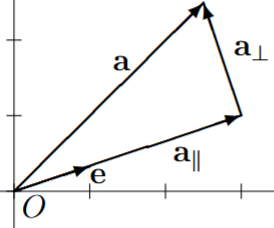
\includegraphics[width=0.1\textwidth]{figures/components.png}                                             \\
        \textbf{Einheitsvektor}       & $\vec{a}_{\parallel} = <\vec{e},\vec{a}> \vec{e}$                                                         \\
                                      & $\vec{a}_{\perp} = \vec{a} - <\vec{e},\vec{a}> \vec{e}$                                                   \\
        \textbf{Cauchy-Schwarz:}      & $||\vec{a}|| ||\vec{b}|| \geq <\vec{a},\vec{b}>$                                                          \\
                                      & gleich wenn $\vec{a} \perp \vec{b}$                                                                       \\
        \textbf{Einheitsnormalvektor} & $||\vec{n_0}|| = \frac{\vec{n}}{||\vec{n}||}$                                                             \\
    \end{tblr}

    \subsection{Normalvektor}
    $\vec{n}=\begin{pmatrix}n_1\\n_2\end{pmatrix}$...Normalvektor, $a=(a_1,a_2)$...Punkt\\

    \begin{align*}
        n_1x + n_2y & = c               \\
        c           & = a_1n_1 + a_2n_2
    \end{align*}
    \subsubsection{Hsse'sche Normalform}
    Normalvektor zum Einheitsnormalvektor mit der Länge 1 gemacht wird, dann ist $|c|$ der Anstand der Geraden vom Ursprung

    \subsection{Kreuzprodukt}
    Wenn $\vec{a}$ und $\vec{b}$ linear unabhaengig (nicht parallel) \\
    $<(\vec{a} \times \vec{b}),\vec{a}> = 0$ bzw. $(\vec{a} \times \vec{b})\perp \vec{b}$\\
    Wenn linear abhängig (parallel)\\
    $\vec{a} =\textit{k}\vec{b}$ oder $\vec{b} =\textit{k}\vec{a}$ $\vec{a} \times \vec{b} = 0$

    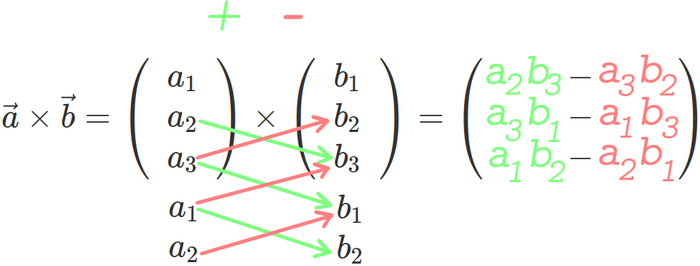
\includegraphics[width=0.17\textwidth]{figures/kreuzprodukt.png}\\
    \subsubsection{Regeln für $\vec{a},\vec{b} \in \mathbb{R}^3$ und $\textit{k,h} \in \mathbb{R}$}
    \begin{align*}
        \vec{a} \times \vec{b}                          & = -\vec{b} \times \vec{a} \\
        (\textit{k}\vec{a}) \times \vec{b}               & = \textit{k}(\vec{a} \times \vec{b}) \\
        (\textit{k}\vec{a}+\textit{h}\vec{b}) \times \vec{c} & = \textit{k}(\vec{a} \times \vec{c}) + \textit{h}(\vec{b} \times \vec{c}) \\
        \vec{a} \times (\textit{k}\vec{b} + \textit{h}\vec{c}) & = \textit{k}(\vec{a} \times \vec{b}) + \textit{h}(\vec{a} \times \vec{c}) \\
        ||\vec{a} \times \vec{b}||                      & = ||\vec{a}|| ||\vec{b}|| \sin(\alpha) \\
    \end{align*}
    wobei $\alpha$ der Winkel zwischen $\vec{a}$ und $\vec{b}$ ist





    \subsection{Orthogonalentwicklung}
    \[<\vec{a},\vec{b}> = \frac{<\vec{a},\vec{b}>}{||\vec{b}||^2}\vec{b}\]
    Wenn $||b||$ = 1, dann ist das Ergebnis
    \[<\vec{a},\vec{b}> = <\vec{a},\vec{b}> \vec{b}\]

    \[<\vec{a}_{\perp},\vec{b}> = 0\]


    \section{Matrix}
    \subsection{Lineare Abbildungen von Matritzen}
    m x n - Matrix -> m Zeilen n Spalten
    V,W...Vektorräume über $\mathbb{R}$ bzw. $\mathbb{C}$
    F:V $\rightarrow$ W heißt linear, wenn  \[f(a\vec{v}+b\vec{u})=af\vec{v}+bf(\vec{u}),  	\forall \vec{v}, \vec{u}  \in V, \forall a, b  \in \mathbb{R}\]
    F:$\mathbb{R}^n \rightarrow \mathbb{R}^m $ kann dargestellt werden in der Form:
    \[f(\vec{x})=\begin{pmatrix}x_1\\x_2\\ \vdots \\x_n\end{pmatrix}=\begin{pmatrix}a_{11}x_1+a_{12}x_2+\cdots+a_{1n}x_n\\a_{21}x_1+a_{22}x_2+\cdots+a_{2n}x_n\\\vdots\\\vdots\\a_{m1}x_1+a_{m2}x_2+\cdots+a_{mn}x_n\end{pmatrix}\]=\[\begin{pmatrix}a_{11} & a_{12} & \cdots & a_{1n}\\a_{21} & a_{22} & \cdots & a_{2n}\\\vdots & \vdots & \ddots & \vdots\\a_{m1} & a_{m2} & \cdots & a_{mn}\end{pmatrix}\begin{pmatrix}x_1\\x_2\\\vdots\\x_n\end{pmatrix}\]
    \[f(\vec{x})=A\vec{x}\] jede Abbildungen $\vec{x} \rightarrow A\vec{x}$ heißt lineare Abbildung

    \subsection{Matrix transformieren}
    Um eine Matrix zu transformieren
    \[A=\begin{pmatrix}a_{11} & a_{12} & \cdots & a_{1n}\\a_{21} & a_{22} & \cdots & a_{2n}\\\vdots & \vdots & \ddots & \vdots\\a_{m1} & a_{m2} & \cdots & a_{mn}\end{pmatrix}\]

    \subsection{Einheitsmatrix}
    \[\mathds{1}=E=\begin{pmatrix}1 & 0 & \cdots & 0\\0 & 1 & \cdots & 0\\\vdots & \vdots & \ddots & \vdots\\0 & 0 & \cdots & 1\end{pmatrix}\]
    \[\mathds{1}A=A\mathds{1}=A\]
    \[AA^{-1}=A^{-1}A=\mathds{1}\]

    \subsection{Quadratische Gleichungen}
    \[ax^2+bx+c=0\]
    \[x_{1,2}= \frac{ -b \pm \sqrt{b^2-4ac}}{2a} \]



    Felix Erlacher, \href{http://erlacher.org/}{http://erlacher.org/}
\end{multicols}

\end{document}
